\documentclass[border=2pt]{standalone}
\usepackage[T1]{fontenc}\usepackage{lmodern}\usepackage{amsmath}
\usepackage{tikz}
\usetikzlibrary{positioning,fit,arrows.meta,calc,backgrounds}
\definecolor{ink}{HTML}{1B1F3B}\definecolor{acc}{HTML}{4B3FA8}\definecolor{org}{HTML}{E08A1E}
\definecolor{teal}{HTML}{2A8C82}\definecolor{red}{HTML}{C0392B}\definecolor{pale}{HTML}{EEF0F8}
\begin{document}
\footnotesize
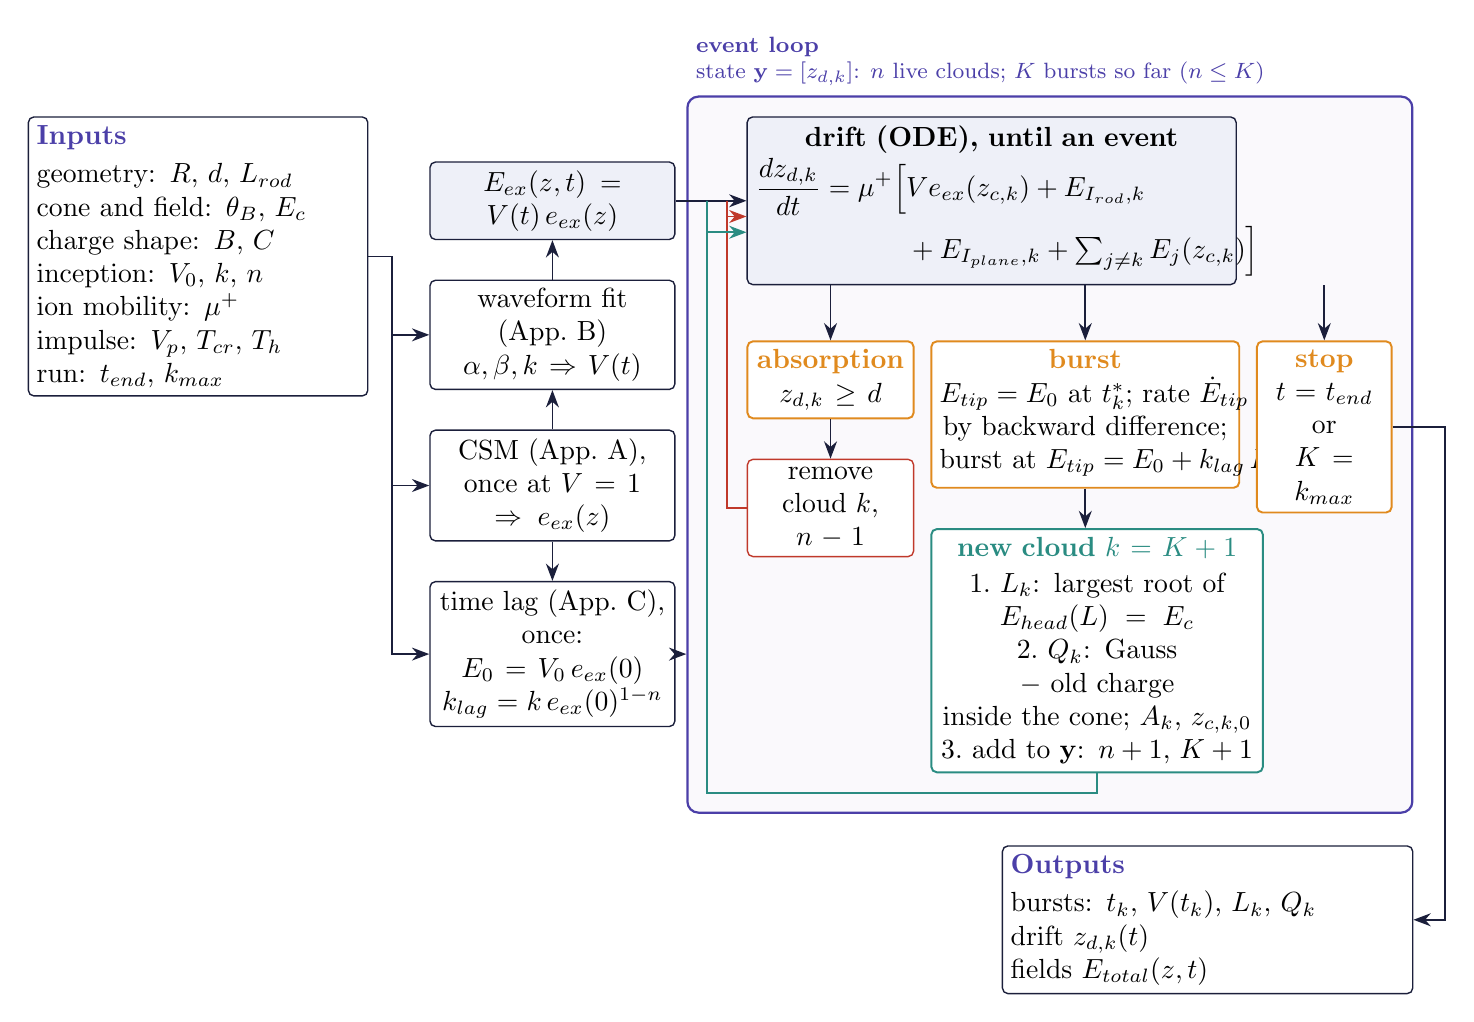
\begin{tikzpicture}[
  node distance=4mm and 6mm, >={Stealth[length=2.2mm]},
  box/.style={draw=ink, rounded corners=2pt, align=center, inner sep=3pt, fill=white, line width=0.5pt},
  ttl/.style={font=\footnotesize\bfseries, text=acc},
  ev/.style={box, draw=org, line width=0.7pt},
  arr/.style={->, draw=ink, line width=0.6pt}]

% inputs
\node[box, align=left, text width=41mm] (in) {%
  {\bfseries\color{acc}Inputs}\\[2pt]
  geometry: $R$, $d$, $L_{rod}$\\
  cone and field: $\theta_B$, $E_c$\\
  charge shape: $B$, $C$\\
  inception: $V_0$, $k$, $n$\\
  ion mobility: $\mu^{+}$\\
  impulse: $V_p$, $T_{cr}$, $T_h$\\
  run: $t_{end}$, $k_{max}$};

% loop: drift first (position reference)
\node[box, fill=pale, text width=60mm, right=48mm of in.north east, anchor=north west] (drift) {%
  {\bfseries drift (ODE), until an event}\\[1pt]
  $\begin{aligned}\frac{dz_{d,k}}{dt}=\mu^{+}\Big[&V e_{ex}(z_{c,k})+E_{I_{rod},k}\\&+E_{I_{plane},k}+\textstyle\sum_{j\neq k}E_{j}(z_{c,k})\Big]\end{aligned}$};

% precompute: E_ex level with drift, CSM and waveform below it
\node[box, fill=pale, text width=29mm, left=9mm of drift] (eex) {$E_{ex}(z,t)=$\\ $V(t)\,e_{ex}(z)$};
\node[box, text width=29mm, below=5mm of eex] (wav) {waveform fit (App.~B)\\ $\alpha,\beta,k \Rightarrow V(t)$};
\node[box, text width=29mm, below=5mm of wav] (csm) {CSM (App.~A), once at $V=1$\\ $\Rightarrow e_{ex}(z)$};
\draw[arr] (csm) -- (wav); \draw[arr] (wav) -- (eex);
\node[box, text width=29mm, below=5mm of csm] (lag) {time lag (App.~C),\\ once:\\ $E_0=V_0\,e_{ex}(0)$\\ $k_{lag}=k\,e_{ex}(0)^{1-n}$};
\draw[arr] (csm) -- (lag);
\coordinate (bus) at ($(in.east)+(3mm,0)$);
\draw[draw=ink, line width=0.6pt] (in.east) -- (bus);
\draw[arr] (bus) |- (wav.west);
\draw[arr] (bus) |- (csm.west);
\draw[arr] (bus) |- (lag.west);
\draw[arr] (eex.east) -- ($(drift.west)+(0,0)$);

\node[ev, text width=19mm, below=7mm of drift.south west, anchor=north west] (ab) {{\bfseries\color{org}absorption}\\ $z_{d,k}\ge d$};
\node[ev, text width=37mm, right=2mm of ab.north east, anchor=north west] (bu) {{\bfseries\color{org}burst}\\ \mbox{$E_{tip}=E_0$ at $t^{*}_k$; rate $\dot{E}_{tip}$}\\ \mbox{by backward difference;}\\ \mbox{burst at $E_{tip}=E_0+k_{lag}\,\dot{E}^{\,n}_{tip}(t^{*}_k)$}};
\node[ev, text width=15mm, right=2mm of bu.north east, anchor=north west] (st) {{\bfseries\color{org}stop}\\ $t=t_{end}$ or\\ $K=k_{max}$};
\node[box, draw=red, text width=19mm, below=5mm of ab] (rm) {remove cloud $k$, $n-1$};
\node[box, draw=teal, line width=0.7pt, text width=40mm, below=5mm of bu.south west, anchor=north west] (nc) {%
  {\bfseries\color{teal}new cloud $k=K+1$}\\[1pt] 1.\ $L_k$: largest root of\\ $E_{head}(L)=E_c$\\ 2.\ $Q_k$: Gauss $-$ old charge\\ inside the cone; $A_k$, $z_{c,k,0}$\\ 3.\ add to $\mathbf{y}$: $n+1$, $K+1$};
\draw[arr] (drift.south -| bu) -- (bu.north);
\draw[arr] (drift.south -| ab) -- (ab.north);
\draw[arr] (drift.south -| st) -- (st.north);
\draw[arr] (bu) -- (bu |- nc.north);
\draw[arr] (ab) -- (rm);
% feedback to drift (up the left side)
\coordinate (fbo) at ($(drift.west)+(-5mm,0)$);
\coordinate (fbi) at ($(drift.west)+(-2.5mm,0)$);
\draw[arr, draw=red] (rm.west) -| (fbi) |- ($(drift.west)+(0,-2mm)$);
\draw[arr, draw=teal] (nc.south) -- ++(0,-2.5mm) -| (fbo) |- ($(drift.west)+(0,-4mm)$);
\coordinate (lowpt) at ($(nc.south)+(0,-2.5mm)$);
\begin{scope}[on background layer]
\node[draw=acc, rounded corners=4pt, line width=0.8pt, fill=acc!3, inner sep=2.5mm, fit=(drift)(bu)(ab)(st)(nc)(rm)(fbo)(lowpt), label={[ttl, anchor=south west, align=left]north west:{event loop\\ {\normalfont state $\mathbf{y}=[z_{d,k}]$: $n$ live clouds; $K$ bursts so far ($n\le K$)}}}] (loop) {};
\end{scope}
\draw[arr] (lag.east) -- (lag.east -| loop.west);

% outputs (below the loop, right-aligned)
\node[box, align=left, text width=50mm, below=4mm of loop.south east, anchor=north east] (out) {%
  {\bfseries\color{acc}Outputs}\\[2pt] bursts: $t_k$, $V(t_k)$, $L_k$, $Q_k$\\ drift $z_{d,k}(t)$\\ fields $E_{total}(z,t)$};
\draw[arr] (st.east) -| ($(loop.east)+(4mm,0)$) |- (out.east);
\end{tikzpicture}
\end{document}
